\section{发展路线图}\label{sec:roadmap}
\begin{figure}[t]
    \centering
    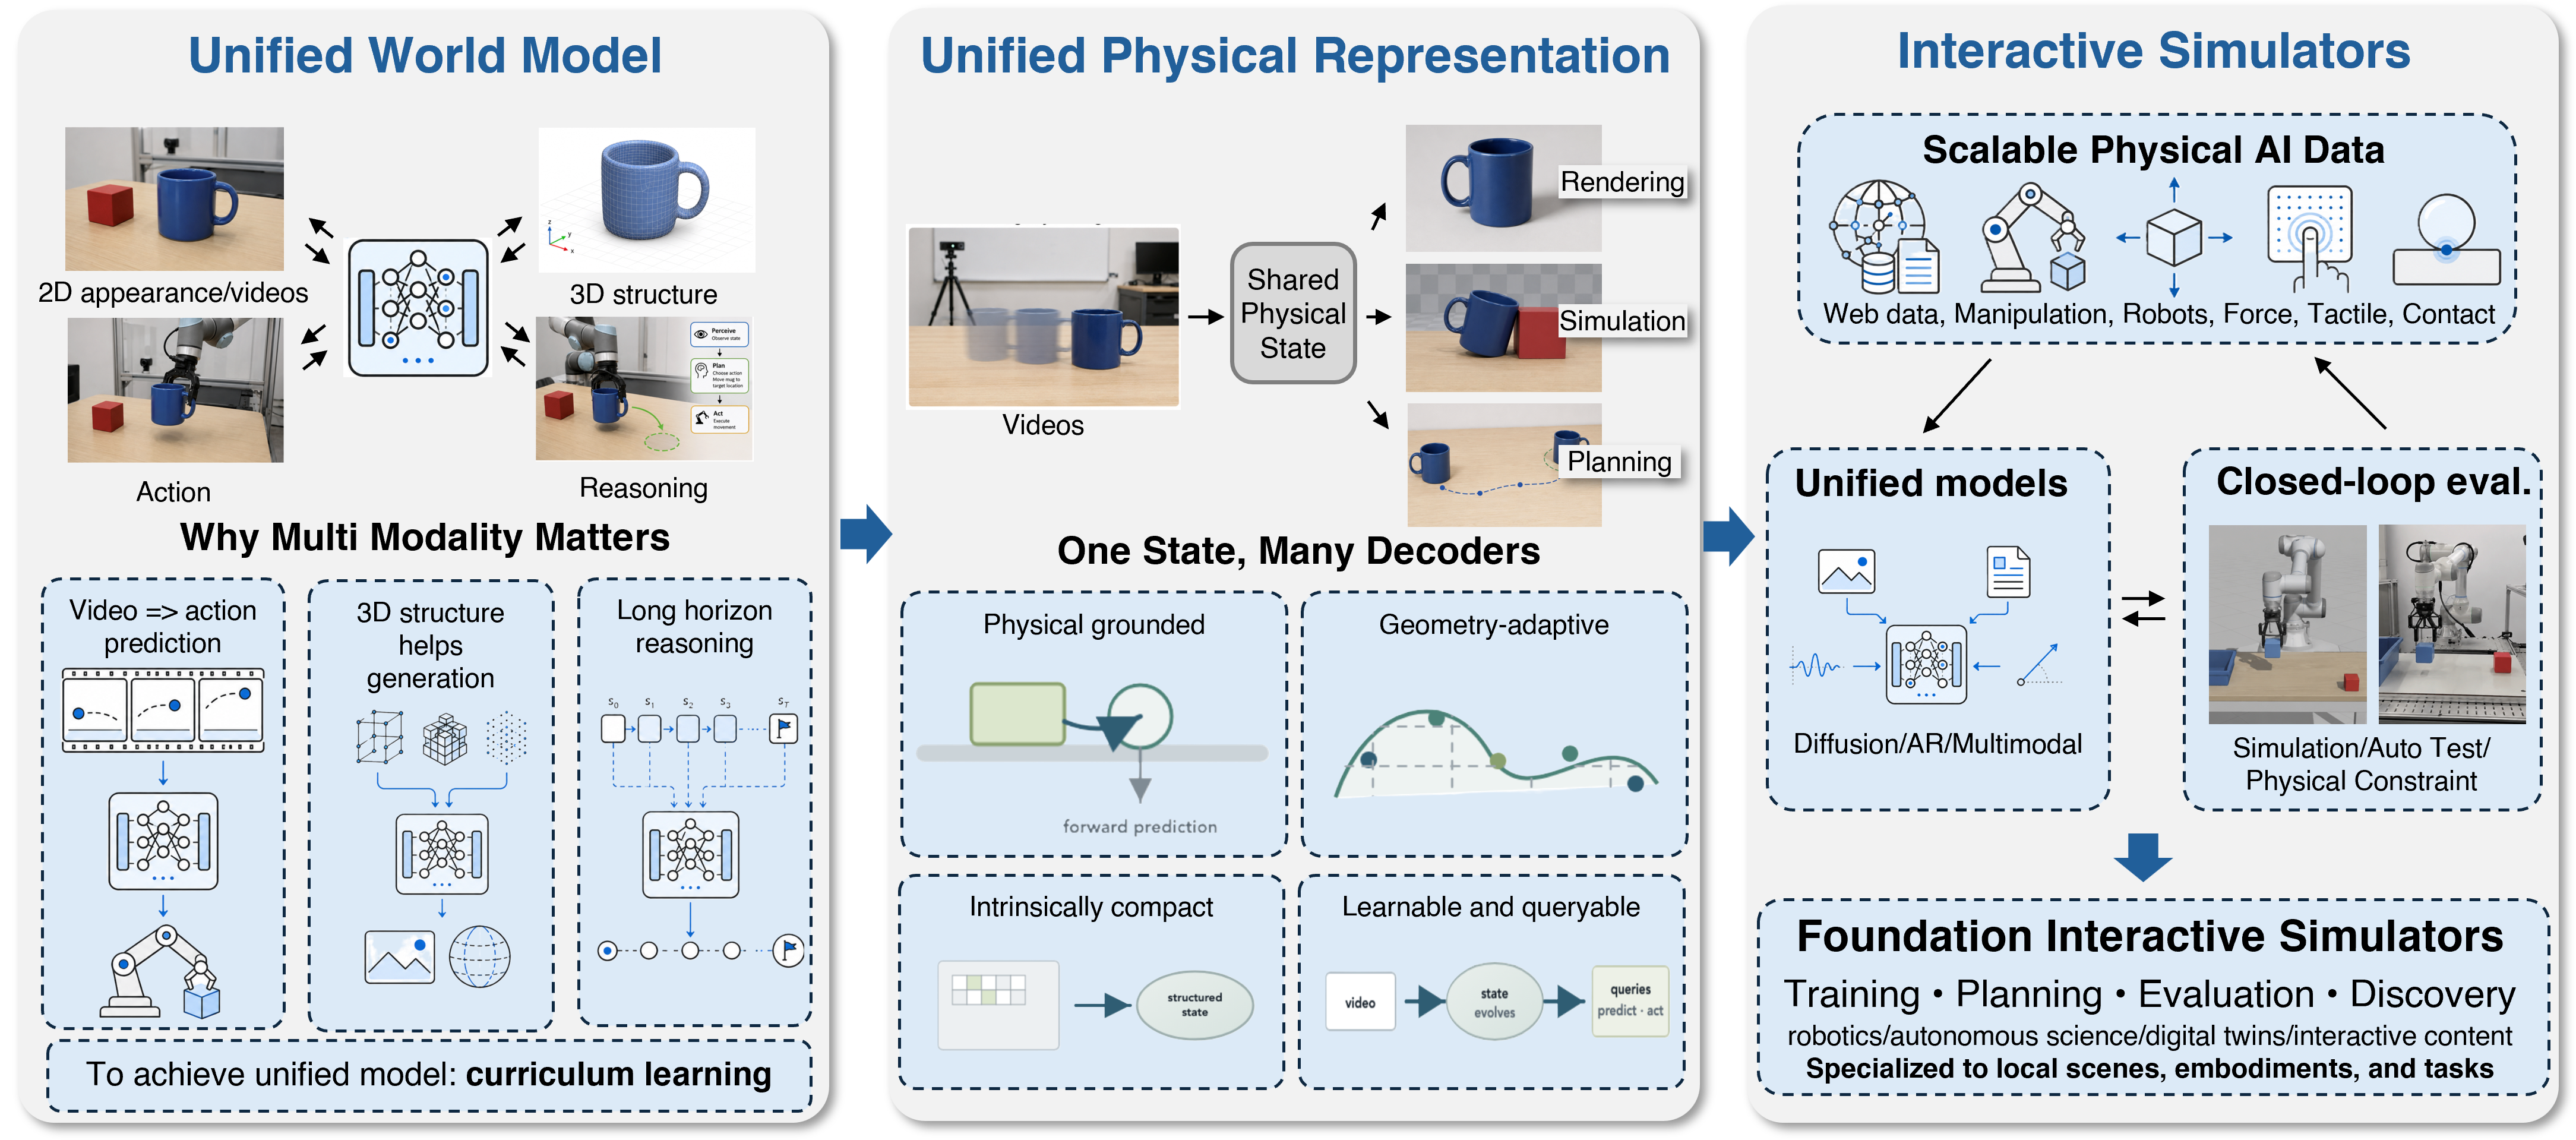
\includegraphics[width=\linewidth]{figs/future2.png}
    \caption{发展下一代世界模型的分阶段路线图。}
    \label{fig:roadmap}
\end{figure}

基于前述讨论，构建未来鲁棒的物理世界模型，需要经过图\ref{fig:roadmap}所示的三个递进阶段。首先，世界模型必须利用多种统一模态，整合各类异步采样信号，使模型能够在大多数物理环境中工作。其次，必须将这些不同模态提炼为统一物理表征（Unified Physical Representation），即单一、高度压缩的内部状态；各种下游任务都能直接从这一状态解码出渲染、模拟与规划。第三，结合先进架构与具有物理依据的数据，扩展这些表征，进而实现基础模型规模的交互模拟器（Foundation-Scale Interactive Simulator）。在这一最终阶段，世界模型成为闭环、可复用环境，允许智能体在真实执行之前安全地探索、评估和改进行动。

\subsection{迈向统一多模态世界模型}
统一多模态是未来世界模型的中心问题，因为准确预测要求共同表示外观、空间结构、状态、行动和长时域推理。视频捕捉运动，三维结构支持视角一致的记忆，行动—状态信号解释可控变化，语义推理把局部预测与长期目标联系起来。因此，统一世界模型不应只是合并模态，还应将这些信号与世界变化方式关联起来。统一多模态对这一问题至关重要，原因有以下几点。

第一，长时域推理需要多模态信息。虽然视频扩散模型能生成可信未来，但操作等许多任务需要长期未来规划，单纯视频扩散模型在有限计算资源下可能难以实现。因此，模型需要搜索、策略或价值信号，在生成分支之间选择。基于扩散的控制系统常将生成与树搜索或行动策略配对\citep{huang2025forgetree,chi2023diffusionpolicy}。引入更多模态后，模型在长期感知、预测与行动选择方面具有更大扩展潜力。

第二，三维等模态能够提供有益补充，在数据稀缺时改善泛化。机器人与驾驶数据集很少覆盖智能体可能遇到的所有相机视角、物体姿态或空间配置。稀疏视角重建与具有几何依据的视频生成，可以合成缺失视角、姿态，以及运动一致的样本，用于训练或测试可控模型\citep{yu2020pixelnerf,liu2023zero123,kang2026geonvs}。这使多模态成为改善泛化的实际途径，因为没有任何单一模态能够充分覆盖罕见空间情况。

第三，行动与状态信号将视频预测从被动预报转化为具身预测。仅凭视觉观测，不能确定哪种抓取会成功，因为同一场景在推、抓取或不行动后，可能产生不同未来。近期视频—行动世界模型，将视觉上下文与显式行动和状态输入结合\citep{zhou2026tau0wm,alradi2026aeroworld}。这说明，仅有视觉规模还不够；模型还必须编码使变化可控的变量。

实际可行的路径，是将统一视为课程（curriculum），而非单一混合词元流。训练可以从静态表征学习开始，用JEPA等图像目标建立语义特征\citep{assran2023ijepa}；随后加入视频、状态、行动和具身数据，同时用紧凑潜在行动，将可控变化与背景外观分离\citep{bruce2024genie,bi2025motus}。

\subsection{迈向统一物理表征}
如前所述，信息压缩是实现统一世界模型的关键。为了将高维感官观测压缩为保留物理世界结构的共享内部状态，表征选择比任何单个渲染器、模拟器或规划器的选择都更重要。然而，当前多数系统维持三种彼此分离的世界定义：渲染采用辐射场或高斯基元等以外观为中心的基元\citep{mildenhall2020nerf,kerbl20233dgaussians}；模拟采用网格或粒子；规划采用占据栅格（occupancy grid）或物体槽位。它们之间的转换有损且缺乏统一原则。因此，必须同时支持感知、模拟与控制的世界模型，会提出这些解码器尚未回答的前置问题：三者究竟可以从哪一种单一内部状态解码出来？

最有希望的长期方向，不是孤立地改进渲染器、模拟器或规划器，而是建立一种\emph{共享物理表征}，使每种功能都成为对它的解码操作。这一表征应具有以下性质。首先，它应有物理依据、可用于模拟，使同一状态承载前向预测所需的动力学与接触结构，而不只是表面外观。其次，它应适应几何差异，容纳真实场景中异构、不规则的几何，而不强加规则栅格或固定模板。此外，它应内在紧凑，编码结构化状态而非稠密场，使容量用于缓慢变化、与决策相关的物理因素，而非像素级细节。在这种表征下，几何、运动、材料属性、外观、语义身份、不确定性与交互状态，将共同编码于一个持续保持的状态中；渲染、模拟与规划不再需要三种独立世界定义，而成为对同一压缩物理状态的不同解码操作：解码为像素或泼溅基元以渲染，解码为形变、应力与接触变量以模拟，或解码为“物体—部件—可供性”结构以规划行动。

这种“一个状态，多个解码器”原则已有部分先例。例如，PhysGaussian\citep{xie2024physgaussian}从同一组高斯核驱动物理模拟与渲染。更广泛的挑战，是设计同时满足各项要求的统一表征：1）能够解码外观、有模拟依据、适应不同几何且紧凑；2）能够从互联网规模视觉数据学习，并将这些数据压缩为持续保持的物理状态；3）该状态能够通过解析或所学动力学演化，并通过任务专用查询接口提供感知预测、反事实模拟与控制。具体采用何种基础结构，仍是开放问题。归根结底，通往物理世界模型的中心问题是：\textit{怎样一种紧凑内部结构，能够保留足够的物理与语义信息，以支持具身智能的所有下游投影？}

\subsection{基础模型规模的交互模拟器}
最后，世界模型的另一用途，是构建支持行动想象、任务生成、反馈整合或持续改进的交互模拟器。世界模型有助于扩大模拟器规模，提供可复用环境，使智能体与科学系统能够在真实实验之前测试行动、评估风险并探索可能结果。

这一愿景受到大语言模型和近期视频生成模型规模扩展成功的启发：更大模型、更广泛数据与更多计算，带来了推理和泛化能力的系统性提升。这给世界模型提出中心问题：物理动力学能否出现类似尺度行为？更具体地说，更大的模型、更多样的数据、可扩展的交互训练数据集，以及物理信息丰富的标注，能否提高世界模型维持物理一致性、预测长时域动力学、可靠响应智能体行动并充当交互模拟器的能力？

为实现这一目标，需要考虑三个关键方面。首先，需要可扩展模型架构，同时支持高保真世界预测与可靠的行动条件交互。近期扩散和流匹配模型能够生成高质量视觉未来，自回归及大语言模型式架构在长上下文序列建模和推理方面具有优势。Cosmos 3等较新的统一多模态模型，以及Bernini等规划器—渲染器框架进一步表明，语言、视觉、视频、音频和行动可以在更加统一的建模框架中被处理或协调。对基础模型规模交互模拟器而言，关键架构问题仍然开放：什么样的模型设计，能够在引入力、触觉反馈、接触状态及本体感觉等更丰富物理模态的同时，扩展可控交互能力？

其次，基础模型规模交互模拟器的发展，既依赖互联网视频，也依赖可扩展物理数据集的构建。互联网视频引入通用视觉与行动先验；第一人称操作视频以行动或手部运动标注补充；真实机器人轨迹提供具有物理依据的控制信号。除这些来源外，更丰富的物理监督同样重要，包括三维状态、物体运动、接触事件、力、触觉反馈、热信号和材料属性。

第三，物理交互模拟器必须在闭环场景中检验。学习得到的模拟器可以为策略训练与评估提供低成本交互环境，但其自身预测仍须根据真实结果或可靠物理约束验证。因此，未来系统需要超越视觉可信性的评估规程，度量预测未来是否与行动保持因果一致，能否在长时域保持一致，以及能否预测机器人或人工智能驱动自主湿实验室中的真实执行结果。
